\section{Slotted\-Mac Class Reference}
\label{classSlottedMac}\index{SlottedMac@{SlottedMac}}
A protocol which divides time into discrete slots during which packets can be transmitted.  


{\tt \#include $<$mac\_\-protocol.hpp$>$}

Inheritance diagram for Slotted\-Mac::\begin{figure}[H]
\begin{center}
\leavevmode
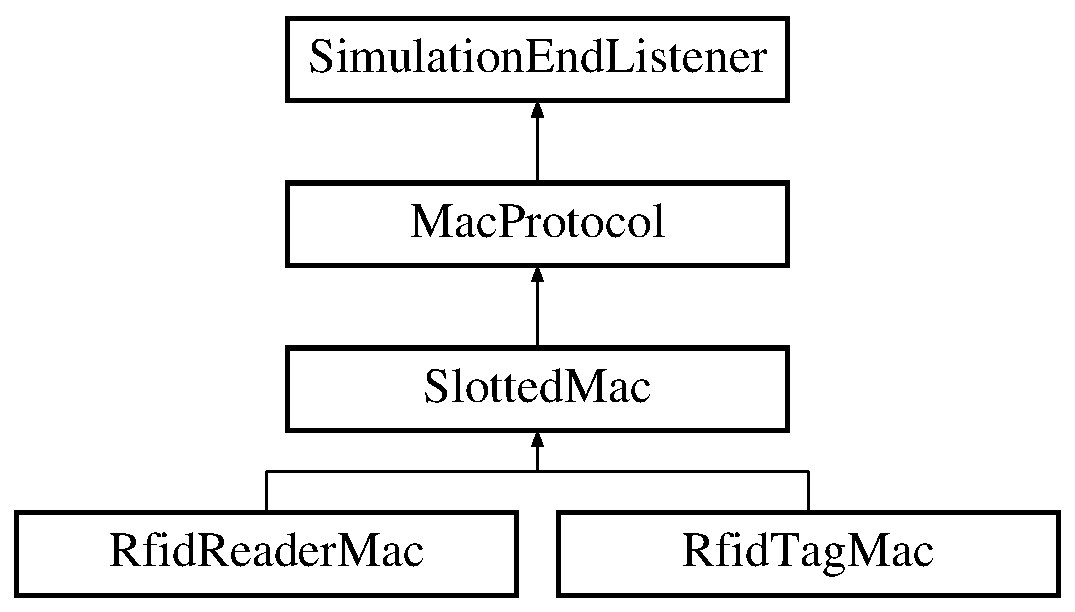
\includegraphics[height=4cm]{classSlottedMac}
\end{center}
\end{figure}
\subsection*{Public Types}
\begin{CompactItemize}
\item 
typedef boost::shared\_\-ptr$<$ \bf{Slotted\-Mac} $>$ \bf{Slotted\-Mac\-Ptr}\label{classSlottedMac_2017056aae90ca668491d299866cb0e9}

\begin{CompactList}\small\item\em Smart pointer that clients should use. \item\end{CompactList}\end{CompactItemize}
\subsection*{Public Member Functions}
\begin{CompactItemize}
\item 
virtual \bf{$\sim$Slotted\-Mac} ()\label{classSlottedMac_e86bc778598e00329b21f8e5f4ee8b72}

\begin{CompactList}\small\item\em A destructor. \item\end{CompactList}\end{CompactItemize}
\subsection*{Protected Member Functions}
\begin{CompactItemize}
\item 
\bf{Slotted\-Mac} (Node\-Ptr node)\label{classSlottedMac_a5727fe1eaa8d981c02b7870e0bf2fd5}

\begin{CompactList}\small\item\em A constructor. \item\end{CompactList}\item 
virtual void \bf{begin\-Slot\-Event} ()=0\label{classSlottedMac_aac32b0a42282f4e2d694200cb392045}

\begin{CompactList}\small\item\em This function is called whenever a slot begins. \item\end{CompactList}\item 
void \bf{set\-Slot\-Time} (const \bf{Sim\-Time} \&slot\-Time)
\begin{CompactList}\small\item\em Set the time per slot. \item\end{CompactList}\item 
\bf{Sim\-Time} \bf{get\-Slot\-Time} () const 
\begin{CompactList}\small\item\em Get the time per slot. \item\end{CompactList}\item 
bool \bf{in\-Contention\-Cycle} () const 
\begin{CompactList}\small\item\em Determine whether the node is currently engaged in a contention cycle. \item\end{CompactList}\item 
void \bf{stop\-Contention\-Cycle} ()\label{classSlottedMac_143047c6cae0fdc6b6d15e9ccdb7c048}

\begin{CompactList}\small\item\em Stops a contention cycle by reseting the appropriate state variables to zero. \item\end{CompactList}\end{CompactItemize}
\subsection*{Protected Attributes}
\begin{CompactItemize}
\item 
Timer\-Ptr \bf{m\_\-slot\-Timer}\label{classSlottedMac_5386c5d39426ac98d2647cbfc44a66e1}

\begin{CompactList}\small\item\em A timer for when each slot begins. \item\end{CompactList}\item 
\bf{t\_\-uint} \bf{m\_\-current\-Slot\-Number}\label{classSlottedMac_91232b9266e0c169131934d50bbf19fc}

\begin{CompactList}\small\item\em The current slot number in the cycle. \item\end{CompactList}\item 
\bf{t\_\-uint} \bf{m\_\-tx\-Slot\-Number}\label{classSlottedMac_cb05cd3a34804495a26f07af82245d41}

\begin{CompactList}\small\item\em This object's chosen transmission slot. \item\end{CompactList}\item 
\bf{t\_\-uint} \bf{m\_\-number\-Of\-Slots}
\begin{CompactList}\small\item\em The number of slots in the current contention cycle. \item\end{CompactList}\item 
Packet\-Ptr \bf{m\_\-packet\-To\-Transmit}\label{classSlottedMac_58354b4d36f7c2ffc2317d90425a29ee}

\begin{CompactList}\small\item\em A pointer to the packet to transmit in the chosen slot. \item\end{CompactList}\end{CompactItemize}
\subsection*{Static Protected Attributes}
\begin{CompactItemize}
\item 
static const double \bf{m\_\-DEFAULT\_\-SLOT\_\-TIME} = 2.0e-3\label{classSlottedMac_116f2f50b04d4e50ea6dc752a48435f3}

\begin{CompactList}\small\item\em The default time per slot. \item\end{CompactList}\end{CompactItemize}
\subsection*{Friends}
\begin{CompactItemize}
\item 
class \bf{Slotted\-Mac\-Slot\-Event}\label{classSlottedMac_6df6ba29e30155ace27c25f82e099316}

\end{CompactItemize}


\subsection{Detailed Description}
A protocol which divides time into discrete slots during which packets can be transmitted. 



Definition at line 182 of file mac\_\-protocol.hpp.

\subsection{Member Function Documentation}
\index{SlottedMac@{Slotted\-Mac}!getSlotTime@{getSlotTime}}
\index{getSlotTime@{getSlotTime}!SlottedMac@{Slotted\-Mac}}
\subsubsection{\setlength{\rightskip}{0pt plus 5cm}\bf{Sim\-Time} Slotted\-Mac::get\-Slot\-Time () const\hspace{0.3cm}{\tt  [inline, protected]}}\label{classSlottedMac_eeec78e7a36e51656cdc7c4f8ecdcab5}


Get the time per slot. 

\begin{Desc}
\item[Returns:]the current time per slot. \end{Desc}


Definition at line 237 of file mac\_\-protocol.hpp.

Referenced by Rfid\-Tag\-Mac::begin\-Slot\-Event(), and Rfid\-Reader\-Mac::begin\-Slot\-Event().\index{SlottedMac@{Slotted\-Mac}!inContentionCycle@{inContentionCycle}}
\index{inContentionCycle@{inContentionCycle}!SlottedMac@{Slotted\-Mac}}
\subsubsection{\setlength{\rightskip}{0pt plus 5cm}bool Slotted\-Mac::in\-Contention\-Cycle () const\hspace{0.3cm}{\tt  [inline, protected]}}\label{classSlottedMac_7881edcfa833a795dae7b1bbe21479a1}


Determine whether the node is currently engaged in a contention cycle. 

\begin{Desc}
\item[Returns:]true if the node is in a contention cycle. \end{Desc}


Definition at line 247 of file mac\_\-protocol.hpp.

References m\_\-current\-Slot\-Number, and m\_\-number\-Of\-Slots.

Referenced by Rfid\-Reader\-Mac::end\-Request\-Cycle\-Event(), Rfid\-Tag\-Mac::handle\-Recvd\-Upper\-Layer\-Packet(), and Rfid\-Tag\-Mac::handle\-Request\-Packet().\index{SlottedMac@{Slotted\-Mac}!setSlotTime@{setSlotTime}}
\index{setSlotTime@{setSlotTime}!SlottedMac@{Slotted\-Mac}}
\subsubsection{\setlength{\rightskip}{0pt plus 5cm}void Slotted\-Mac::set\-Slot\-Time (const \bf{Sim\-Time} \& {\em slot\-Time})\hspace{0.3cm}{\tt  [inline, protected]}}\label{classSlottedMac_8c2f671fe54da66a7a930db211239018}


Set the time per slot. 

\begin{Desc}
\item[Parameters:]
\begin{description}
\item[{\em slot\-Time}]the new time per slot. \end{description}
\end{Desc}


Definition at line 228 of file mac\_\-protocol.hpp.

Referenced by Rfid\-Reader\-Mac::Rfid\-Reader\-Mac(), and Rfid\-Tag\-Mac::Rfid\-Tag\-Mac().

\subsection{Member Data Documentation}
\index{SlottedMac@{Slotted\-Mac}!m_numberOfSlots@{m\_\-numberOfSlots}}
\index{m_numberOfSlots@{m\_\-numberOfSlots}!SlottedMac@{Slotted\-Mac}}
\subsubsection{\setlength{\rightskip}{0pt plus 5cm}\bf{t\_\-uint} \bf{Slotted\-Mac::m\_\-number\-Of\-Slots}\hspace{0.3cm}{\tt  [protected]}}\label{classSlottedMac_69376c02ac9cd637729a72241beafbb9}


The number of slots in the current contention cycle. 

If m\_\-current\-Slot\-Number $<$ m\_\-number\-Of\-Slots, then the node is not currently engaged in a contention cycle. 

Definition at line 208 of file mac\_\-protocol.hpp.

Referenced by Rfid\-Tag\-Mac::begin\-Slot\-Event(), Rfid\-Reader\-Mac::begin\-Slot\-Event(), Rfid\-Reader\-Mac::handle\-Packet\-Sent(), Rfid\-Tag\-Mac::handle\-Recvd\-Upper\-Layer\-Packet(), Rfid\-Tag\-Mac::handle\-Request\-Packet(), in\-Contention\-Cycle(), Rfid\-Reader\-Mac::start\-Next\-Contention\-Cycle(), and stop\-Contention\-Cycle().

The documentation for this class was generated from the following files:\begin{CompactItemize}
\item 
mac\_\-protocol.hpp\item 
mac\_\-protocol.cpp\end{CompactItemize}
